\chapter*{Capitolo 3}
\addcontentsline{toc}{chapter}{Capitolo 3}

\section*{Descrizione del progetto}
\addcontentsline{toc}{section}{Descrizione del progetto}
Nella parte progettuale sono state usate e analizzate le tecnologie DPDK e P4 sul piano dell'inoltro dati. Lo scopo del progetto è infatti quello di trovare un modo per velocizzare l'instradamento dei pacchetti su degli switch P4. Per studiare i possibili modi per migliorare l'instradamento, prima sono stati svolti dei test di trasmissione tra due host usando solo DPDK e successivamente tra due host utilizzando solo P4. Alla fine sono stati registrati i risultati e confrontati a livello numerico, per avere un paragone tra le performance delle due tecnologie a livello di forwarding.
\newline
\\
La parte di progetto di DPDK ha come scopo quello di analizzare le performance della suite di librerie DPDK, in ambiente virtualizzato e ``Bare Metal". Per la generazione e la ricezione di pacchetti è stato usato il tool Pktgen DPDK \cite{wiles_pktgen_2022}.
La dimensione dei pacchetti è per tutti i test di 1500 byte.
\newline
\\
La parte di progetto riguardante P4 ha lo scopo di studiare le prestazioni di ricezione dati degli switch P4, più precisamente sfruttando il target BMv2. I test si riferiscono a un host interno ad una macchina virtuale. Le interfacce sono collegate tramite delle Veth passando per uno o più switch P4.
Gli switch P4 hanno un programma che fa accept e forward dei pacchetti, mentre gli host sono collocati su due namespaces differenti.

\section*{Sviluppo del progetto: DPDK}
\addcontentsline{toc}{section}{Sviluppo del progetto: DPDK}

\subsection*{Setup}
\addcontentsline{toc}{subsection}{Setup}
Per avere un supporto ai Poll Mode Drivers, è necessario abilitare l'apposito Kernel driver.
VFIO-PCI è un Kernel driver che permette un accesso diretto al dispositivo grazie alle sue API. È consigliato per l'uso con DPDK perché supporta l' IOMMU \cite{noauthor_iommu}, elemento essenziale per la comunicazione delle CPU con le periferiche, e può sfruttare il PCI Passthrough \cite{noauthor_pci_passthrough}, ovvero può collegarsi direttamente al dispositivo fisico PCI, rendendo le prestazioni ancora migliori.
Se si è impossibilitati ad abilitare VFIO, si può comunque usare il modulo standard \textbf{uio\_pci\_generic} incluso nel Kernel Linux, che però presenta qualche limitazione, poiché non supporta la creazione di funzioni virtuali.
È inoltre possibile fare il setup delle hugepages e successivamente disattivare la scheda di rete per renderla disponibile all'utilizzo. La NIC viene virtualmente separata dal device driver per essere associata a DPDK.\\ Il valore \textbf{02:00.0} corrisponde al PCI address della scheda di rete \cite{noauthor_6_nodate}.
I comandi con prefisso ``dpdk" fanno parte della suite fornita con l'applicativo. Per elencare le schede disponibili è possibile utilizzare
\begin{minted}{bash}
sudo dpdk-devbind.py -s
\end{minted}
Oppure manualmente con:
\begin{minted}{bash}
sudo lshw -c network -businfo
\end{minted}
Per velocizzare il setup si possono utilizzare le varie utility fornite dalla suite DPDK per montare le hugepages o fare il binding della scheda di rete.
La configurazione sottostante è la stessa per ogni host su cui eseguiranno le istanze di Pktgen.
\begin{minted}
[frame=lines,
framesep=2mm,
baselinestretch=1.2,
bgcolor=white,
fontsize=\footnotesize,
linenos
]{bash}
#!/bin/bash
modprobe uio
modprobe uio_pci_generic
dpdk-hugepages.py -p 1G --setup 2G
ifconfig enp2s0 down
dpdk-devbind.py -b uio_pci_generic 02:00.0
\end{minted}

\subsection*{Pktgen DPDK}
\addcontentsline{toc}{subsection}{Pktgen DPDK}
DPDK Pktgen è un generatore di traffico che sfrutta DPDK a livello Data Plane che permette di creare pacchetti personalizzati di dimensione, IP/MAC source/destination, arbitrari.
Per il corretto funzionamento richiede almeno due core logici. Il core 0 resta in ascolto come ``master" e permette il funzionamento della linea di comando di Pktgen, l'altro esegue la ricezione o la trasmissione come ``slave". Questo tool può essere eseguito anche nella stessa macchina su più istanze, in modo da avere un metodo di test anche all'interno dello stesso host.
Nella interfaccia grafica mostrata in \textbf{{Figura \ref{fig:pktgen_1}}}
 si osserva come sia possibile manipolare i pacchetti generabili specificandone anche il protocollo o il campo dati, mentre in \textbf{{Figura \ref{fig:wireshark}}} si possono notare i diversi pacchetti generati.
Un esempio di esecuzione di pktgen è il seguente
\begin{minted}{bash}
sudo ./pktgen -l 0-4 -n 3 --proc-type auto -- -T -P -m "1.0, 2.1, 3.2, 4.3"
\end{minted}
Dove si specificano i logical cores, i memory channels e le opzioni di EAL. In questo caso il core 1 si occupa della porta 0 RX/TX, il core 2 della porta 1 RX,TX, il core 3 della porta 2 RX/TX e il core 4 della porta 3 RX/TX.
\leavevmode\newline
Il device driver utilizzato per virtualizzare le schede di rete è MacVTap.
\vspace{0.5mm}
\FloatBarrier
\begin{figure}[h]
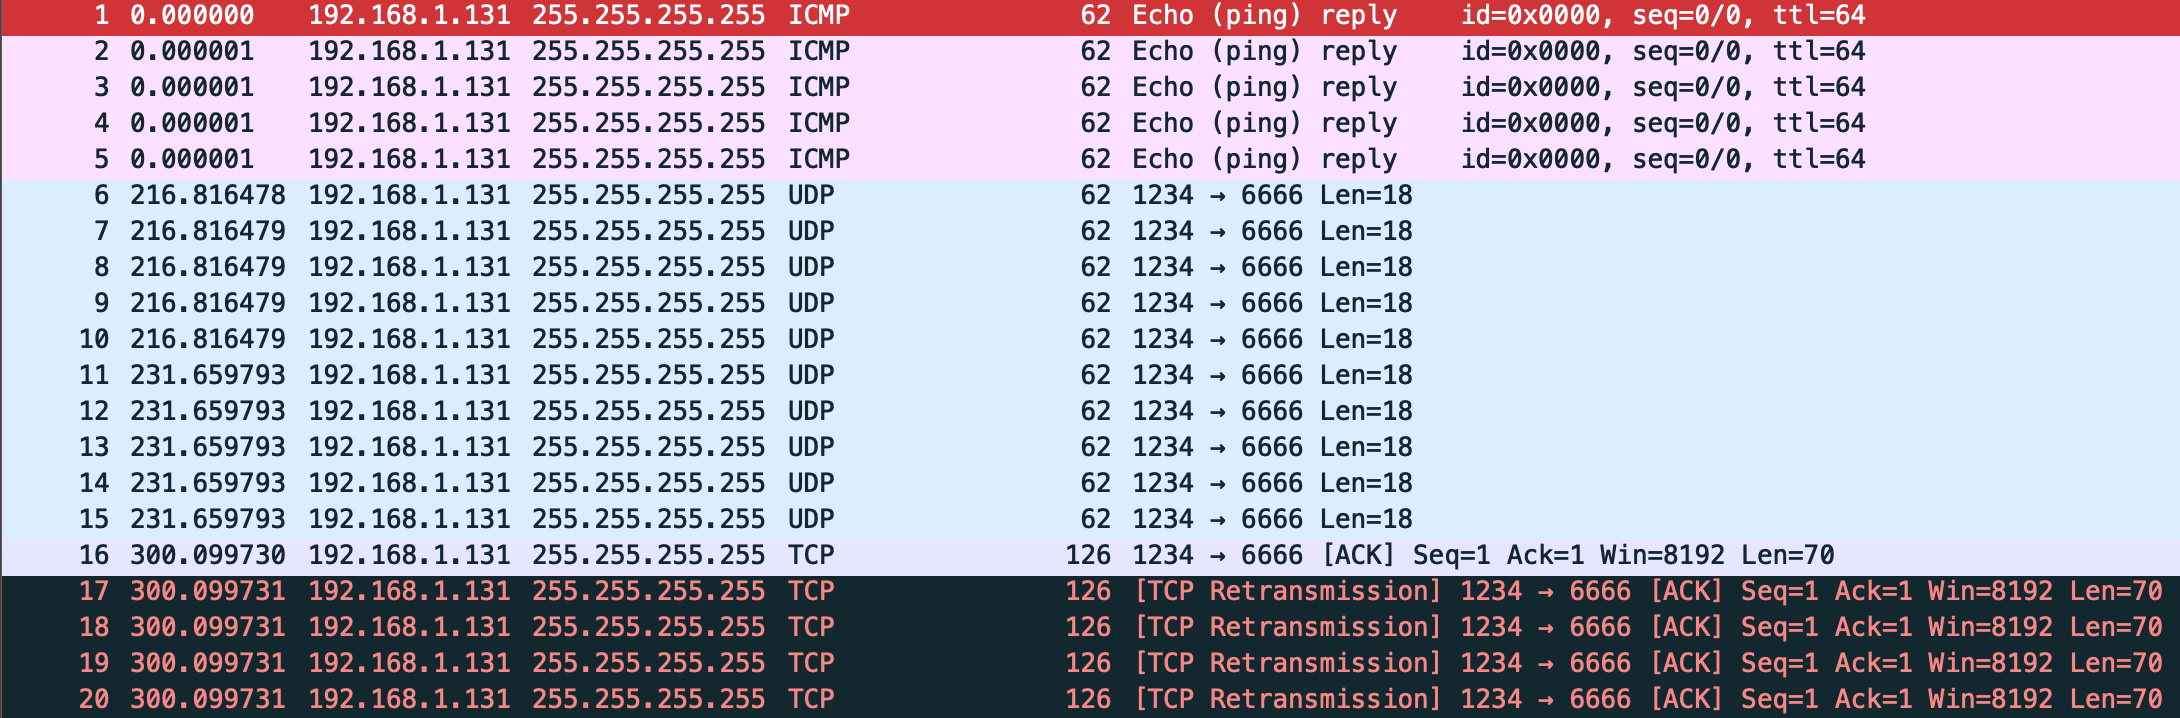
\includegraphics[scale=0.25]{images/wireshark.png} 
\centering
\caption{\textit{Manipolazione dei Pacchetti con Pktgen, analisi con Wireshark}} \cite{noauthor_wireshark_nodate}
\label{fig:wireshark}
\vspace{1cm}
\end{figure}
\FloatBarrier

\FloatBarrier
\begin{figure}[h]
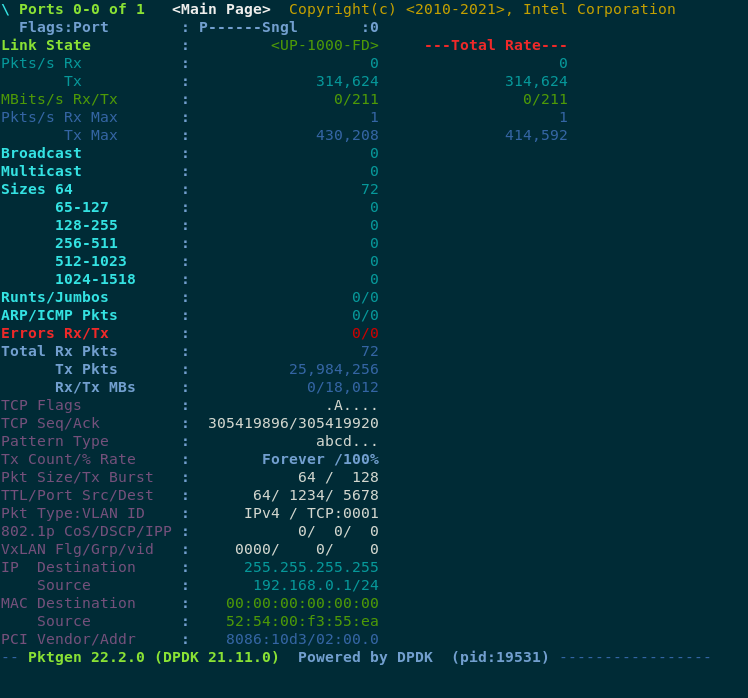
\includegraphics[scale=0.4]{images/pktgen_1.png}
\centering
\caption{\textit{Interfaccia di Pktgen}}
\vspace{1cm}
\label{fig:pktgen_1}
\end{figure}
\FloatBarrier


\section*{Infrastrutture}
\addcontentsline{toc}{subsection}{Infrastrutture}

\subsection*{Test all' interno della stessa Macchina Virtuale}
\addcontentsline{toc}{subsection}{Test all' interno della stessa Macchina Virtuale}
Nell' infrastruttura in \textbf{{Figura \ref{fig:dpdk_vm1}}} il test viene eseguito in una macchina virtuale in cui è presente un unico host, collegato ad una scheda di rete paravirtualizzata. Lo stesso host si mette in ascolto e in ricezione. Sono stati utilizzati in totale 2 core ed il master core.
Il primo core resta in trasmissione (TX) mentre il secondo in ricezione (RX). I due core sono dedicati alla stessa istanza di Pktgen. I test fanno riferimento alla stessa scheda di rete, l'host dispone di 4GB di RAM.
\FloatBarrier
\begin{figure}[h]
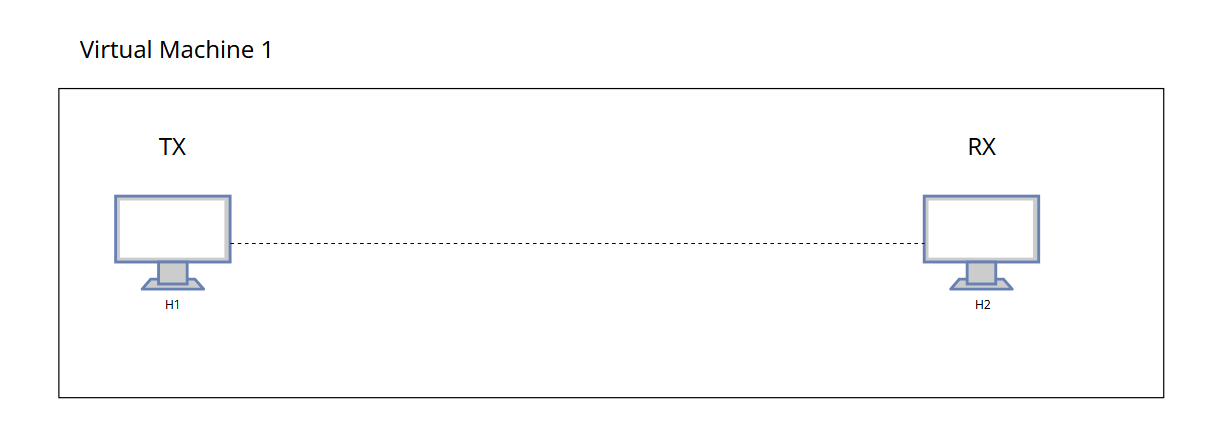
\includegraphics[scale=0.5]{images/dpdk_vm1.png}
\centering
\caption{\textit{Test in macchina virtuale con un unico host}}
\vspace{1cm}
\label{fig:dpdk_vm1}
\end{figure}
\FloatBarrier
\leavevmode\newline
Per configurare le operazioni che deve eseguire il primo core di trasmissione dall'interfaccia di pktgen si può usare la seguente configurazione
\begin{minted}[
frame=lines,
framesep=2mm,
baselinestretch=1.2,
bgcolor=white,
fontsize=\footnotesize,
linenos
]{bash}
set 0 src ip 192.168.100.1/24
set 0 dst ip 192.168.100.1/24
set 0 dst mac 00:00:00:00:00:01
set 0 src mac 00:00:00:00:00:01
set 0 size 64
set 0 pattern user
set 0 user pattern test
\end{minted}

\subsection*{Test tra due Macchine Virtuali}
\addcontentsline{toc}{subsection}{Test tra due Macchine Virtuali}
In \textbf{{Figura \ref{fig:dpdk_vm2}}} il test viene eseguito tra due host in due macchine virtuali collegate in rete interna. I due host sono collegati alla stessa scheda di rete fisica, ma virtualmente a due schede di rete paravirtualizzate con due IP e due indirizzi MAC diversi. H1 è l'host che effettua la trasmissione, mentre H2 effettua la ricezione. Sono stati utilizzati in totale 1 core ed il master core per ogni istanza di Pktgen. Ogni host dispone di 4GB di RAM, per un totale complessivo di 8GB.
\FloatBarrier
\begin{figure}[h]
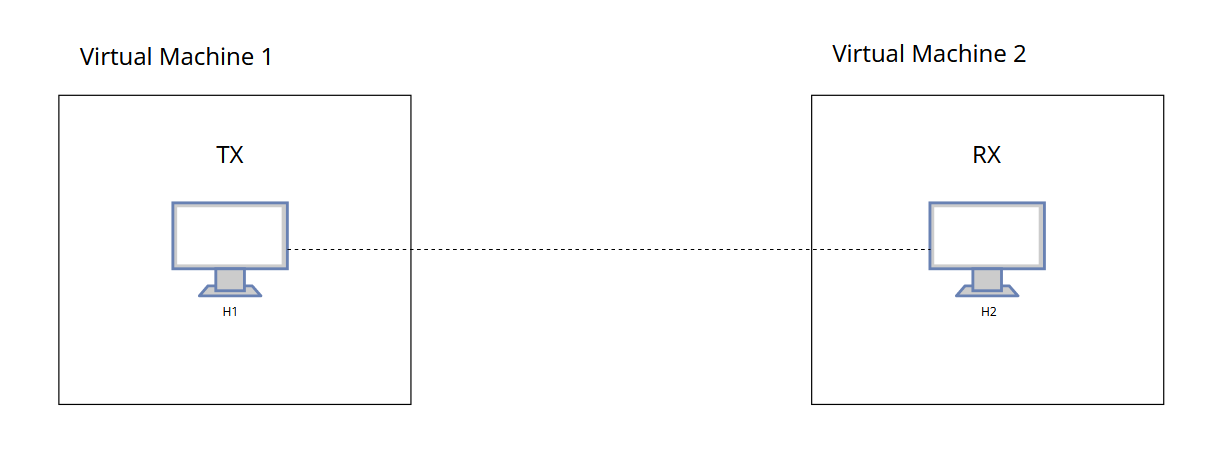
\includegraphics[scale=0.5]{images/dpdk_vm2.png}
\centering
\caption{\textit{Test tra due NIC di due Host in due macchine virtuali}}
\label{fig:dpdk_vm2}
\vspace{1cm}
\end{figure}
\FloatBarrier

In questo caso si specifica l'IP e il MAC del secondo host, in modo da far arrivare i pacchetti a destinazione.
\begin{minted}[
frame=lines,
framesep=2mm,
baselinestretch=1.2,
bgcolor=white,
fontsize=\footnotesize,
linenos
]{bash}
set 0 src ip 192.168.100.1/24
set 0 dst ip 192.168.100.2/24
set 0 dst mac 00:00:00:00:00:01
set 0 src mac 00:00:00:00:00:02
set 0 size 64
set 0 pattern user
set 0 user pattern test
\end{minted}


\subsection*{Test in rete interna in condizioni reali}
\addcontentsline{toc}{subsection}{Test in rete interna in condizioni reali}
La \textbf{{Figura \ref{fig:dpdk_lan2}}} mostra il test effettuato in una rete locale, in cui i due host sono due calcolatori diversi, collegati tra loro da uno switch. In questo caso gli host dispongono di schede di rete fisiche con indirizzi fisici e risiedono all'interno di una rete domestica. H1 è l'host che effettua la trasmissione, mentre H2 effettua la ricezione. Sono stati utilizzati in totale 4 core ed il master core per ogni istanza di Pktgen. Ogni calcolatore dispone di 16GB di RAM.
\FloatBarrier
\begin{figure}[h]
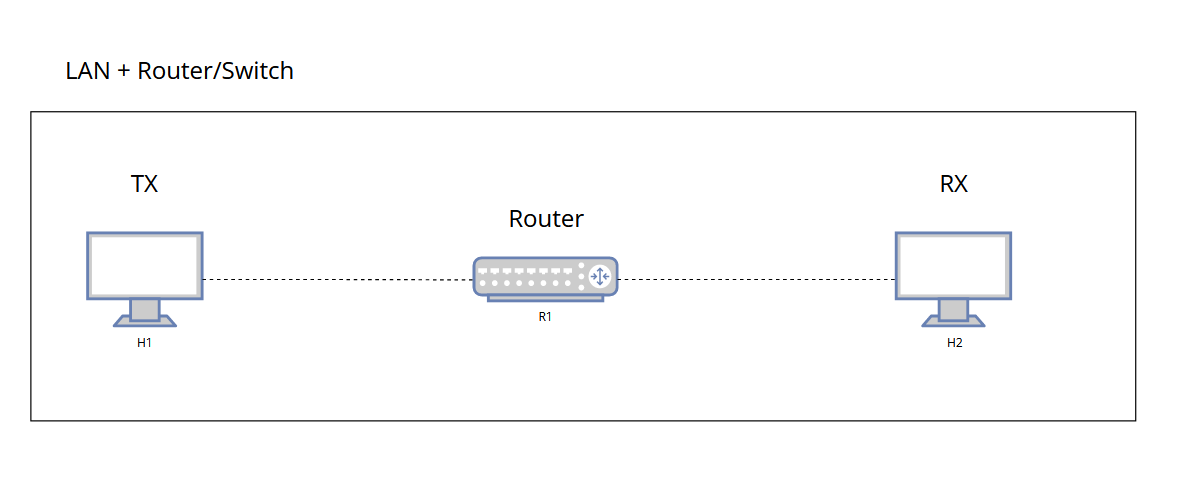
\includegraphics[scale=0.5]{images/dpdk_lan2.png}
\centering
\caption{\textit{Test tra due NIC di due Host nella stessa LAN passando per un Router}}
\vspace{1cm}
\label{fig:dpdk_lan2}
\end{figure}
\FloatBarrier



\begin{minted}[
frame=lines,
framesep=2mm,
baselinestretch=1.2,
bgcolor=white,
fontsize=\footnotesize,
linenos
]{bash}
set 0 src ip 192.168.1.17/24
set 0 dst ip 192.168.1.18/24
set 0 dst mac d8:d3:85:ea:1b:ee
set 0 src mac 00:1b:63:84:45:e6
set 0 size 64
set 0 pattern user
set 0 user pattern test
\end{minted}


\section*{Sviluppo del progetto: P4}
\addcontentsline{toc}{section}{Sviluppo del progetto: P4}

\subsection*{Setup}
\addcontentsline{toc}{subsection}{Setup}
Per creare l'infrastruttura di uno o più switch P4 collegati a due host, si deve per prima cosa disporre di due schede di rete paravirtualizzate. Per avere queste due interfacce di sono stati utilizzati i driver MacVTAP. Una volta create le NIC virtuali, è opportuno creare anche due namespace collegati tramite veth e caricare il programma P4 negli switch. Anche in questa fase di setup ci si è serviti di un software esterno per generare traffico. Questa volta è stato utilizzato IPerf3 \cite{noauthor_iperf_nodate} su protocollo TCP.


\subsection*{Accept e Forward}
\addcontentsline{toc}{subsection}{Accept e Forward}
Il seguente snippet di codice mostra l' Ingress Processing del semplice programma usato per fare Accept e Forward ed è caricato in tutte le configurazioni degli switch \cite{noauthor_p4_2022-1}. La versione utilizzata è P4$_{\mbox{16}}$.
\begin{minted}[
frame=lines,
framesep=2mm,
baselinestretch=1.2,
bgcolor=white,
fontsize=\footnotesize,
linenos
]{c}
control MyIngress(inout headers hdr,
                  inout metadata meta,
                  inout standard_metadata_t standard_metadata) {
    action drop() {
        mark_to_drop(standard_metadata);
    }

    action ipv4_forward(macAddr_t dstAddr, egressSpec_t port) {
        standard_metadata.egress_spec = port;
        hdr.ethernet.srcAddr = hdr.ethernet.dstAddr;
        hdr.ethernet.dstAddr = dstAddr;
        hdr.ipv4.ttl = hdr.ipv4.ttl - 1;
    }

    table ipv4_lpm {
        key = {
            hdr.ipv4.dstAddr: lpm;
        }
        actions = {
            ipv4_forward;
            drop;
            NoAction;
        }
        size = 1024;
        default_action = drop();
    }

    apply {
        if (hdr.ipv4.isValid()) {
            ipv4_lpm.apply();
        }
    }
}
\end{minted}
Le regole di forward saranno aggiunte nei singoli switch in successiva fase di runtime.
\pagebreak

\subsection*{Test di trasmissione tra due host con uno switch P4}
\addcontentsline{toc}{subsection}{Test di trasmissione tra due host con uno switch P4}

Nell'infrastruttura mostrata in \textbf{{Figura \ref{fig:p4_basic}}} si hanno due host collegati tra di loro passanti per uno switch P4.
\FloatBarrier
\begin{figure}[h]
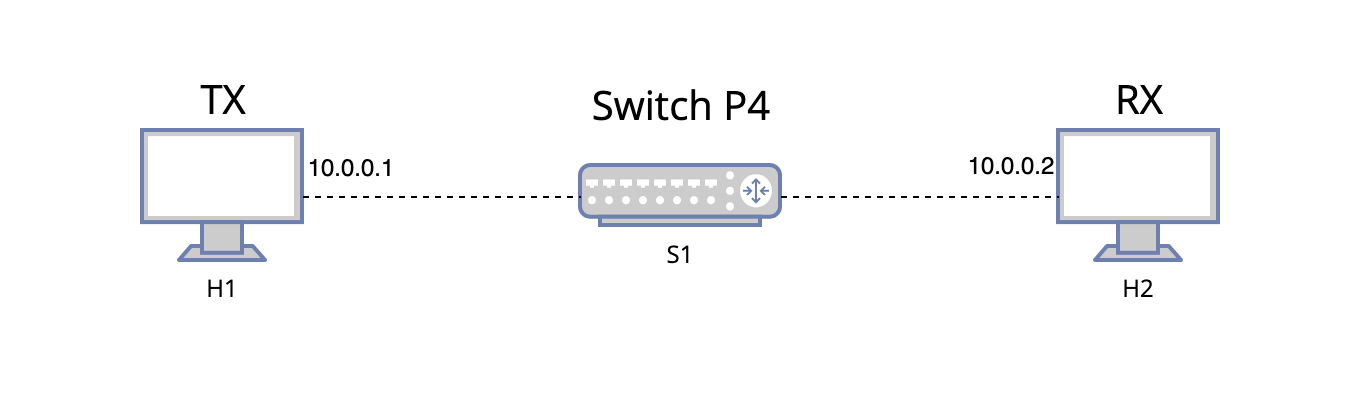
\includegraphics[scale=0.5]{images/p4_basic.png}
\centering
\caption{\textit{Test tra due host passando per uno switch P4}}
\label{fig:p4_basic}
\vspace{1cm}
\end{figure}
\FloatBarrier
\leavevmode\newline
Per avviare il singolo switch si può usare
\begin{minted}[
frame=lines,
framesep=2mm,
baselinestretch=1.2,
bgcolor=white,
fontsize=\footnotesize,
linenos
]{bash}
sudo ./simple_switch -i 1@s1-eth0 -i 2@s1-eth1 basic.json
--thrift-port 9091 --notifications-addr ipc:///tmp/bmv2-1-notifications.ipc
\end{minted}
E poi a runtime per caricare le regole 

\begin{minted}[
frame=lines,
framesep=2mm,
baselinestretch=1.2,
bgcolor=white,
fontsize=\footnotesize,
linenos
]{bash}
table_clear MyIngress.ipv4_lpm
table_add MyIngress.ipv4_lpm MyIngress.ipv4_forward 10.0.0.1/32 => 00:00:00:00:00:01 1
table_add MyIngress.ipv4_lpm MyIngress.ipv4_forward 10.0.0.2/32 => 00:00:00:00:00:01 2
\end{minted}

\subsection*{Test di trasmissione tra due host con due switch P4}
\addcontentsline{toc}{subsection}{Test di trasmissione tra due host con due switch P4}
Nello scenario in \textbf{{Figura \ref{fig:p4_double}}} sono invece presenti due host collegati tra di loro e passanti per due switch P4. Le configurazioni si duplicano rispetto al caso precedente.

\FloatBarrier
\begin{figure}[h]
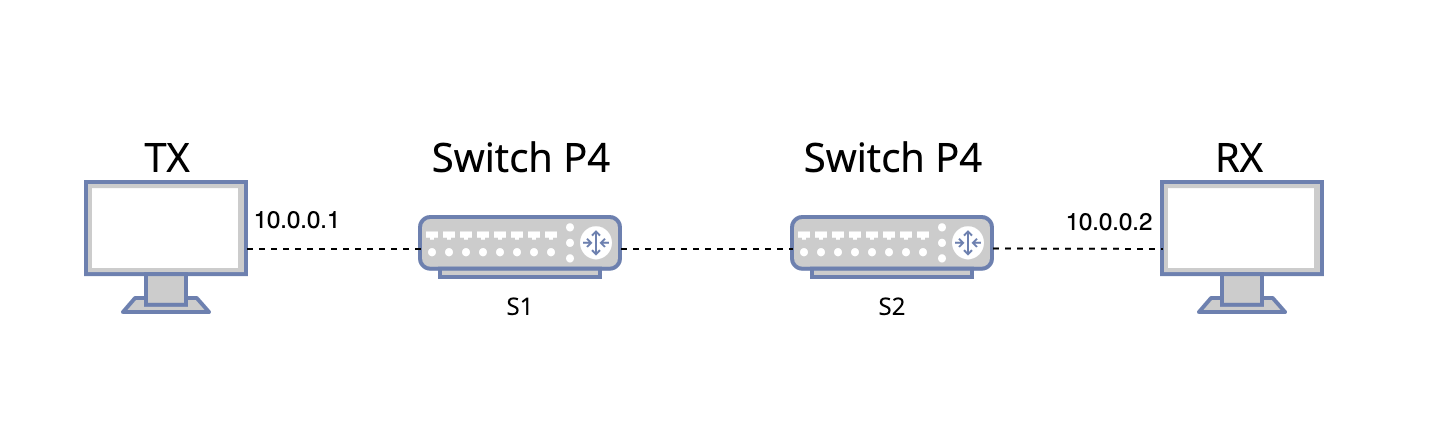
\includegraphics[scale=0.5]{images/p4_double.png}
\centering
\caption{\textit{Test tra due host passando per due switch P4}}
\label{fig:p4_double}
\vspace{1cm}
\end{figure}
\FloatBarrier
\leavevmode\newline
Per caricare le regole sui due switch utilizziamo
\begin{minted}[
frame=lines,
framesep=2mm,
baselinestretch=1.2,
bgcolor=white,
fontsize=\footnotesize,
linenos
]{bash}
sudo ./simple_switch -i 1@s1-eth0 -i 2@s1-eth1 basic.json
--thrift-port 9091 --notifications-addr ipc:///tmp/bmv2-1-notifications.ipc
sudo ./simple_switch -i 1@s2-eth0 -i 2@s2-eth1 basic.json 
--thrift-port 9092 --notifications-addr ipc:///tmp/bmv2-2-notifications.ipc
\end{minted}
La configurazione a runtime diventa la seguente 
\subsubsection*{Switch S1}
\begin{minted}[
frame=lines,
framesep=2mm,
baselinestretch=1.2,
bgcolor=white,
fontsize=\footnotesize,
linenos
]{bash}
table_clear MyIngress.ipv4_lpm
table_add MyIngress.ipv4_lpm MyIngress.ipv4_forward 10.0.0.1/32 => 00:00:00:00:00:01 1
table_add MyIngress.ipv4_lpm MyIngress.ipv4_forward 10.0.0.2/32 => 00:00:00:00:00:02 2
\end{minted}
\subsubsection*{Switch S2}
\begin{minted}[
frame=lines,
framesep=2mm,
baselinestretch=1.2,
bgcolor=white,
fontsize=\footnotesize,
linenos
]{bash}
table_clear MyIngress.ipv4_lpm
table_add MyIngress.ipv4_lpm MyIngress.ipv4_forward 10.0.0.2/32 => 00:00:00:00:00:03 1
table_add MyIngress.ipv4_lpm MyIngress.ipv4_forward 10.0.0.1/32 => 00:00:00:00:00:04 2
\end{minted}